\hypertarget{ne-579-homework-number-2-data-statistics}{%
\section{NE 579 Homework Number 2: Data
Statistics}\label{ne-579-homework-number-2-data-statistics}}

\hypertarget{import-required-libraries}{%
\subsection{Import required libraries}\label{import-required-libraries}}

\begin{lstlisting}[language=Python]
%matplotlib inline
import matplotlib.pyplot as plt
import seaborn as sns
import pandas as pd
import numpy as np
import scipy.io as sio
from scipy.stats import trim_mean, skew, kurtosis, norm
\end{lstlisting}

\begin{lstlisting}
/Users/jrpowers-luhn/miniconda3/envs/579/lib/python3.6/importlib/_bootstrap.py:219: RuntimeWarning: numpy.dtype size changed, may indicate binary incompatibility. Expected 96, got 88
  return f(*args, **kwds)
\end{lstlisting}

\begin{lstlisting}[language=Python]
sns.color_palette('coolwarm')
\end{lstlisting}

\begin{lstlisting}
[(0.40442129049411762, 0.53464349044705883, 0.93200191263529408),
 (0.60316206791764704, 0.73152747735294121, 0.99956527853725485),
 (0.78672070135686278, 0.84480721036862749, 0.93981038494901958),
 (0.93066859633333332, 0.81887699965490202, 0.75914639069803924),
 (0.96731651566666665, 0.65747082880784313, 0.53816015072941181),
 (0.88464343869411766, 0.41001709788235297, 0.32250654924705885)]
\end{lstlisting}

\hypertarget{load-the-data-from-the-file}{%
\subsection{Load the data from the
file}\label{load-the-data-from-the-file}}

\begin{lstlisting}[language=Python]
fn = 'hwkdata.mat'
data_dict = sio.loadmat(fn)
print(data_dict.keys())
\end{lstlisting}

\begin{lstlisting}
dict_keys(['__header__', '__version__', '__globals__', 'x', 'y'])
\end{lstlisting}

\begin{lstlisting}[language=Python]
data_dict['x'].shape
\end{lstlisting}

\begin{lstlisting}
(252, 14)
\end{lstlisting}

\begin{lstlisting}[language=Python]
data_dict['y'].shape
\end{lstlisting}

\begin{lstlisting}
(252, 1)
\end{lstlisting}

\begin{lstlisting}[language=Python]
data = np.append(data_dict['x'], data_dict['y'], 1)
\end{lstlisting}

\begin{lstlisting}[language=Python]
data.shape
\end{lstlisting}

\begin{lstlisting}
(252, 15)
\end{lstlisting}

Now the 2-d array \passthrough{\lstinline!data!} contains 252 samples,
each with 14 input variables and 1 output variable

I will want to label the columns later\ldots{}

\begin{lstlisting}[language=Python]
parameter_names = [
    'Age',
    'Weight',
    'Height',
    'Adiposity Index',
    'Neck circumference',
    'Chest circumference',
    'Abdomen circumference',
    'Hip circumference',
    'Thigh circumference',
    'Knee circumference',
    'Ankle circumference',
    'Extended bicep circumference',
    'Forearm circumference',
    'Wrist circumference',
    '% Bodyweight'
]
\end{lstlisting}

\hypertarget{calculate-statistical-properties-of-the-data}{%
\subsection{Calculate statistical properties of the
data:}\label{calculate-statistical-properties-of-the-data}}

\begin{itemize}
\tightlist
\item
  Maximum
\item
  Minimum
\item
  Mean
\item
  Median
\item
  20\% trimmed mean
\item
  Standard deviation
\item
  Variance
\item
  Skewness
\item
  Kurtosis
\end{itemize}

\hypertarget{maximum}{%
\subsubsection{Maximum}\label{maximum}}

\begin{lstlisting}[language=Python]
np.max(data, axis=0)
\end{lstlisting}

\begin{lstlisting}
array([  81.  ,  363.15,   77.75,   48.9 ,   51.2 ,  136.2 ,  148.1 ,
        147.7 ,   87.3 ,   49.1 ,   33.9 ,   45.  ,   34.9 ,   21.4 ,
         45.1 ])
\end{lstlisting}

\hypertarget{minimum}{%
\subsubsection{Minimum}\label{minimum}}

\begin{lstlisting}[language=Python]
np.min(data, axis=0)
\end{lstlisting}

\begin{lstlisting}
array([  22. ,  118.5,   29.5,   18.1,   31.1,   79.3,   69.4,   85. ,
         47.2,   33. ,   19.1,   24.8,   21. ,   15.8,    0. ])
\end{lstlisting}

\hypertarget{mean}{%
\subsubsection{Mean}\label{mean}}

\begin{lstlisting}[language=Python]
np.mean(data, axis=0)
\end{lstlisting}

\begin{lstlisting}
array([  44.88492063,  178.92440476,   70.14880952,   25.43690476,
         37.99206349,  100.82420635,   92.55595238,   99.9047619 ,
         59.40595238,   38.59047619,   23.10238095,   32.2734127 ,
         28.66388889,   18.2297619 ,   18.93849206])
\end{lstlisting}

\hypertarget{median}{%
\subsubsection{Median}\label{median}}

\begin{lstlisting}[language=Python]
np.median(data, axis=0)
\end{lstlisting}

\begin{lstlisting}
array([  43.  ,  176.5 ,   70.  ,   25.05,   38.  ,   99.65,   90.95,
         99.3 ,   59.  ,   38.5 ,   22.8 ,   32.05,   28.7 ,   18.3 ,   19.  ])
\end{lstlisting}

\hypertarget{trimmed-mean}{%
\subsubsection{20\% Trimmed Mean}\label{trimmed-mean}}

\begin{lstlisting}[language=Python]
trim_mean(data, 0.2, axis=0)
\end{lstlisting}

\begin{lstlisting}
array([  44.44078947,  176.55361842,   70.25      ,   25.05986842,
         37.92894737,  100.12763158,   91.80789474,   99.32828947,
         59.13092105,   38.49144737,   22.91381579,   32.16118421,
         28.69934211,   18.21776316,   18.86578947])
\end{lstlisting}

\hypertarget{standard-deviation}{%
\subsubsection{Standard Deviation}\label{standard-deviation}}

\begin{lstlisting}[language=Python]
np.std(data, axis=0)
\end{lstlisting}

\begin{lstlisting}
array([ 12.57701082,  29.3307901 ,   3.65558099,   3.64086527,
         2.4260852 ,   8.41373177,  10.76166054,   7.14982914,
         5.2395251 ,   2.4070145 ,   1.69152717,   3.0152732 ,
         2.01667787,   0.93173074,   7.73546169])
\end{lstlisting}

\hypertarget{variance}{%
\subsubsection{Variance}\label{variance}}

\begin{lstlisting}[language=Python]
np.var(data, axis=0)
\end{lstlisting}

\begin{lstlisting}
array([ 158.18120118,  860.29524766,   13.36327239,   13.25589994,
          5.88588939,   70.79088231,  115.81333759,   51.12005669,
         27.4526233 ,    5.79371882,    2.86126417,    9.09187248,
          4.06698964,    0.86812217,   59.83736757])
\end{lstlisting}

\hypertarget{skewness}{%
\subsubsection{Skewness}\label{skewness}}

\begin{lstlisting}[language=Python]
skew(data, axis=0)
\end{lstlisting}

\begin{lstlisting}
array([ 0.28183067,  1.19807685, -5.35287991,  1.55239101,  0.54932508,
        0.6774921 ,  0.83341904,  1.48820106,  0.81631331,  0.51366304,
        2.24168861,  0.28382759, -0.21802506,  0.27993485,  0.14338879])
\end{lstlisting}

\hypertarget{kurtosis}{%
\subsubsection{Kurtosis}\label{kurtosis}}

\begin{lstlisting}[language=Python]
kurtosis(data, axis=0)
\end{lstlisting}

\begin{lstlisting}
array([ -0.43193939,   5.14182358,  58.34569713,   6.55632326,
         2.64223799,   0.94408639,   2.18073601,   7.30021682,
         2.5894009 ,   1.01687492,  11.68578418,   0.46494688,
         0.82550054,   0.36415485,  -0.32445733])
\end{lstlisting}

\hypertarget{also-calculate-kurt---3}{%
\paragraph{\texorpdfstring{Also calculate
\(Kurt - 3\)}{Also calculate Kurt - 3}}\label{also-calculate-kurt---3}}

\begin{lstlisting}[language=Python]
kurtosis(data, axis=0) - 3 * np.ones_like(kurtosis(data, axis=0))
\end{lstlisting}

\begin{lstlisting}
array([ -3.43193939,   2.14182358,  55.34569713,   3.55632326,
        -0.35776201,  -2.05591361,  -0.81926399,   4.30021682,
        -0.4105991 ,  -1.98312508,   8.68578418,  -2.53505312,
        -2.17449946,  -2.63584515,  -3.32445733])
\end{lstlisting}

\hypertarget{difference-between-mean-and-median}{%
\paragraph{Difference between mean and
median}\label{difference-between-mean-and-median}}

\begin{lstlisting}[language=Python]
with sns.color_palette('coolwarm'):
    f = plt.figure()
    s = np.divide(np.mean(data, axis=0) - np.median(data, axis=0), np.std(data, axis=0))
    ax = plt.subplot(121)
    plt.bar(np.arange(s.shape[0]), s, label=r'$\mu$ - median')
    #plt.bar(np.arange(s.shape[0]), np.mean(data, axis=0) - np.median(data, axis=0), label=r'$\mu$ - median')
    #plt.bar(np.arange(s.shape[0]), kurtosis(data, axis=0) / kurtosis(data, axis=0).max(axis=0),
    #        alpha=0.5, label='Kurtosis')
    #plt.bar(np.arange(s.shape[0]), skew(data, axis=0),
    #        alpha=0.5, label='Skewness')
    plt.legend(loc="upper right")
    plt.savefig('images/mu_minus_median.png', dpi=300, bbox_inches='tight')
    plt.show()
\end{lstlisting}

\begin{figure}
\centering
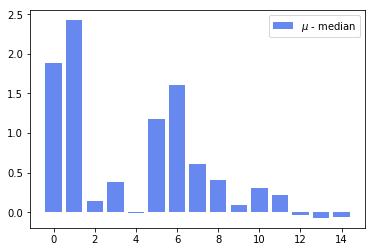
\includegraphics{output_35_0.png}
\caption{png}
\end{figure}

From this plot we see that the mean (sensitive to outliers) exceeds the
median (insensitive to outliers)

\begin{lstlisting}[language=Python]
with sns.color_palette('coolwarm'):
    plt.bar(np.arange(np.mean(data, axis=0).shape[0]),
        np.divide(np.mean(data, axis=0) - trim_mean(data, 0.2, axis=0), np.std(data, axis=0)), label=r'$\mu$ - trim mean')
    plt.legend(loc='upper right')
    #plt.bar(np.arange(trim_mean(data, 0.2, axis=0).shape[0]),
    #        trim_mean(data, 0.2, axis=0))
    plt.savefig('images/mu_minus_trimmed_mean.png', dpi=300, bbox_inches='tight')
    plt.show()
\end{lstlisting}

\begin{figure}
\centering
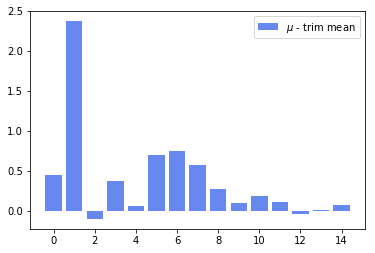
\includegraphics{output_37_0.png}
\caption{png}
\end{figure}

\begin{lstlisting}[language=Python]
with sns.color_palette('coolwarm'):
    f = plt.figure()
    ax1 = f.add_subplot(121)
    ax1.bar(np.arange(np.mean(data, axis=0).shape[0]),
            np.divide(np.mean(data, axis=0) - trim_mean(data, 0.2, axis=0),
                      np.std(data, axis=0)), 
            label=r'$\mu$ - trim mean')
    ax1.legend(loc='lower center')
    
    ax2 = f.add_subplot(122, sharey=ax1)
    s = np.divide(np.mean(data, axis=0) - np.median(data, axis=0), np.std(data, axis=0))
    ax2.bar(np.arange(s.shape[0]), s, label=r'$\mu$ - median')
    plt.setp(ax2.get_yticklabels(), visible=False)
    plt.legend(loc="lower center")
    
    plt.setp(ax1.get_xticklabels(), visible=False)
    plt.setp(ax2.get_xticklabels(), visible=False)
    
    ax1.set_xlabel('Parameter number')
    ax2.set_xlabel('Parameter number')
    
    plt.savefig('images/robust_statistics.png', dpi=300, bbox_inches='tight')
    
\end{lstlisting}

\begin{figure}
\centering
\includegraphics{output_38_0.png}
\caption{png}
\end{figure}

\hypertarget{now-look-at-covariance-and-correlation}{%
\section{Now look at covariance and
correlation}\label{now-look-at-covariance-and-correlation}}

\begin{lstlisting}[language=Python]
plt.figure(figsize=(20,20))
sns.heatmap(np.corrcoef(data.T), vmin=-1, vmax=1, center=0, cmap='coolwarm',
            square=True, annot=True)
plt.savefig('images/correlation_heatmap.png', dpi=300, bbox_inches='tight')
plt.show()
\end{lstlisting}

\begin{figure}
\centering
\includegraphics{output_40_0.png}
\caption{png}
\end{figure}

\begin{lstlisting}[language=Python]
\end{lstlisting}

\begin{lstlisting}[language=Python]
\end{lstlisting}

\hypertarget{pandas}{%
\section{Pandas}\label{pandas}}

\begin{lstlisting}[language=Python]
stat_names = [
    "Parameter", "Max", "Min", "Mean", "Median", "20% Trimmed Mean",
    "Standard Deviation", "Variance", "Skewness", "Kurtosis"
]
\end{lstlisting}

\begin{lstlisting}[language=Python]
summary_statistics = pd.DataFrame(columns=stat_names)
summary_statistics['Parameter'] = parameter_names
summary_statistics['Max'] = np.max(data, axis=0)
summary_statistics['Min'] = np.min(data, axis=0)
summary_statistics['Mean'] = np.mean(data, axis=0)
summary_statistics['Median'] = np.median(data, axis=0)
summary_statistics['20% Trimmed Mean'] = trim_mean(data, 0.2, axis=0)
summary_statistics['Standard Deviation'] = np.std(data, axis=0)
summary_statistics['Variance'] = np.var(data, axis=0)
summary_statistics['Skewness'] = skew(data, axis=0)
summary_statistics['Kurtosis'] = kurtosis(data, axis=0)
\end{lstlisting}

\begin{lstlisting}[language=Python]
summary_statistics
\end{lstlisting}

Parameter

Max

Min

Mean

Median

20\% Trimmed Mean

Standard Deviation

Variance

Skewness

Kurtosis

0

Age

81.00

22.0

44.884921

43.00

44.440789

12.577011

158.181201

0.281831

-0.431939

1

Weight

363.15

118.5

178.924405

176.50

176.553618

29.330790

860.295248

1.198077

5.141824

2

Height

77.75

29.5

70.148810

70.00

70.250000

3.655581

13.363272

-5.352880

58.345697

3

Adiposity Index

48.90

18.1

25.436905

25.05

25.059868

3.640865

13.255900

1.552391

6.556323

4

Neck circumference

51.20

31.1

37.992063

38.00

37.928947

2.426085

5.885889

0.549325

2.642238

5

Chest circumference

136.20

79.3

100.824206

99.65

100.127632

8.413732

70.790882

0.677492

0.944086

6

Abdomen circumference

148.10

69.4

92.555952

90.95

91.807895

10.761661

115.813338

0.833419

2.180736

7

Hip circumference

147.70

85.0

99.904762

99.30

99.328289

7.149829

51.120057

1.488201

7.300217

8

Thigh circumference

87.30

47.2

59.405952

59.00

59.130921

5.239525

27.452623

0.816313

2.589401

9

Knee circumference

49.10

33.0

38.590476

38.50

38.491447

2.407015

5.793719

0.513663

1.016875

10

Ankle circumference

33.90

19.1

23.102381

22.80

22.913816

1.691527

2.861264

2.241689

11.685784

11

Extended bicep circumference

45.00

24.8

32.273413

32.05

32.161184

3.015273

9.091872

0.283828

0.464947

12

Forearm circumference

34.90

21.0

28.663889

28.70

28.699342

2.016678

4.066990

-0.218025

0.825501

13

Wrist circumference

21.40

15.8

18.229762

18.30

18.217763

0.931731

0.868122

0.279935

0.364155

14

\% Bodyweight

45.10

0.0

18.938492

19.00

18.865789

7.735462

59.837368

0.143389

-0.324457

\begin{lstlisting}[language=Python]
with open('summary_statistics_table.tex', 'w') as f:
    f.write(summary_statistics.to_latex(index=True))
\end{lstlisting}

\begin{lstlisting}[language=Python]
(summary_statistics['Max'] - summary_statistics['Min'] ) / summary_statistics['Standard Deviation']
\end{lstlisting}

0 4.691099 1 8.341064 2 13.198996 3 8.459528 4 8.284952 5 6.762754 6
7.312998 7 8.769440 8 7.653365 9 6.688784 10 8.749490 11 6.699227 12
6.892524 13 6.010320 14 5.830292 dtype: float64

\begin{lstlisting}[language=Python]
summary_statistics['Mean']
\end{lstlisting}

0 44.884921 1 178.924405 2 70.148810 3 25.436905 4 37.992063 5
100.824206 6 92.555952 7 99.904762 8 59.405952 9 38.590476 10 23.102381
11 32.273413 12 28.663889 13 18.229762 14 18.938492 Name: Mean, dtype:
float64

\begin{lstlisting}[language=Python]
props = dict(boxstyle='round', facecolor='wheat', alpha=0.5)
with sns.color_palette('coolwarm'):
    f, ax = plt.subplots(4, 4, figsize=(20,15), sharey=True)
#    for i in range(len(parameter_names)):
    for i in range(4):
        for j in range(4):
            if (i*4+j) < len(parameter_names):
                x = np.linspace(np.min(data[:,i*4+j]), np.max(data[:,i*4+j]))
                y = data[:,i*4+j].shape[0]*norm.pdf(x, loc=np.mean(data[:,i*4+j]), scale=np.std(data[:,i*4+j]))
                ax[i,j].plot(x, y)
                ax[i,j].hist(data[:,i*4+j], bins=15)
                ax[i,j].axvline(x=np.mean(data[:,i*4+j]), linestyle='dotted')
                ax[i,j].set_title(f'{parameter_names[i*4+j]}')
                textstr = f'Skewness {skew(data[:,i*4+j]):0.2f}\nKurtosis {kurtosis(data[:,i*4+j]):0.2f}'
                ax[i,j].text(0.5, 0.95, textstr, transform=ax[i,j].transAxes,
                             fontsize=14, verticalalignment='top', bbox=props)
plt.savefig('images/histogram_array.png', dpi=300, bbox_inches='tight')
plt.show()
\end{lstlisting}

\begin{figure}
\centering
\includegraphics{output_50_0.png}
\caption{png}
\end{figure}

\begin{lstlisting}[language=Python]
type(parameter_names)
\end{lstlisting}

\begin{lstlisting}[language=Python]
len([1,2])
\end{lstlisting}

\begin{lstlisting}[language=Python]
N = [5, 25, 100, 250]
D = [norm.rvs(size=n) for n in N]

f, axs = plt.subplots(1, len(N), sharey='all')

for _ in range(len(N)):
    axs[_].hist(D[_], density=True)
    axs[_].set_title(f'N={N[_]}')

plt.savefig('sample_size.png', dpi=300, bbox_inches='tight')
plt.show()
\end{lstlisting}

\begin{figure}
\centering
\includegraphics{output_53_0.png}
\caption{png}
\end{figure}

\begin{lstlisting}[language=Python]
\end{lstlisting}

